\documentclass[12pt,spanish]{article}
\usepackage[spanish]{babel}
\usepackage{graphicx}
\usepackage{color}
\usepackage{xcolor}
\usepackage{colortbl}
\usepackage{amsthm,thmtools}
\usepackage{multirow}
\usepackage{amsmath}
\usepackage{subcaption}
\usepackage{adjustbox}
\usepackage{multirow}
\usepackage[hidelinks]{hyperref}
\usepackage{caption}
\usepackage{amsthm}
\usepackage{multicol}
\usepackage[outputdir=build]{minted}
\usepackage{float}
\usepackage{amsfonts}
\usepackage{titling}
\usepackage{soul}
\usepackage{listings}
\usepackage{array}
\graphicspath{ {./img/} {../../LaTeX/img/}}
\selectlanguage{spanish}
\usepackage[utf8]{inputenc}
\usepackage{graphicx}
\usepackage[a4paper,left=3cm,right=2cm,top=2.5cm,bottom=2.5cm]{geometry}


\makeatletter
\patchcmd\thmt@mklistcmd
  {\thmt@thmname}
  {\check@optarg{\thmt@thmname}}
  {}{}
\patchcmd\thmt@mklistcmd
  {\thmt@thmname\ifx}
  {\check@optarg{\thmt@thmname }\ifx}
  {}{}
\protected\def\check@optarg#1{%
  \@ifnextchar\thmtformatoptarg\@secondoftwo{#1}%
}
\makeatother


\newtheorem{definition}{Definición}
\numberwithin{definition}{subsection}
\renewcommand{\listtheoremname}{Índice de definiciones}



\title{Inteligencia Artificial}
\setlength{\droptitle}{10em}
\author{Carlos Sánchez Páez}

\makeindex
\begin{document}


\begin{titlepage}

\newlength{\centeroffset}
\setlength{\centeroffset}{-0.5\oddsidemargin}
\addtolength{\centeroffset}{0.5\evensidemargin}
\thispagestyle{empty}

\noindent\hspace*{\centeroffset}
\begin{minipage}{\textwidth}

\centering

\includegraphics[width=0.9\textwidth]{logo_ugr.jpg}\\[1.4cm]

\textsc{ \Large Inteligencia Artificial\\[0.2cm]}
\textsc{GRADO EN INGENIERÍA INFORMÁTICA}\\[1cm]

{\Huge\bfseries Resumen del temario\\}
\end{minipage}

\vspace{1.5cm}
\noindent\hspace*{\centeroffset}
\begin{minipage}{\textwidth}
\centering

\textbf{Autor}\\ {Carlos Sánchez Páez}\\[2.5ex]

\includegraphics[width=0.3\textwidth]{etsiit_logo.png}\\[0.1cm]
\vspace{1.5cm}

\includegraphics[width=0.5\textwidth]{decsai.jpg}\\[0.1cm]
\vspace{1cm}
\textsc{Escuela Técnica Superior de Ingenierías Informática y de Telecomunicación}\\
\vspace{1cm}
\textsc{Curso 2017-2018}
\end{minipage}
\end{titlepage}
\thispagestyle{empty}
\newpage
\tableofcontents{}
\newpage
\listoffigures
\thispagestyle{empty}
\newpage

\section{Tema 1. Introducción.}

\subsection{¿Qué es la IA?}

En la siguiente tabla podemos observar los cuatro enfoques que se han seguido a lo largo de la historia para definir la IA. Los de la izquierda miden el éxito en términos de la fidelidad en la forma de actuar de los humanos, mientras que los de la derecha toman como referencia la \emph{racionalidad}. Un sistema es reacional si hace "lo correcto'' en función de su conocimiento.
\begin{figure}[H]
\centering
\begin{tabular}{|m{7.5cm}|m{7.5cm}|}
\hline
\textbf{Sistemas que piensan como humanos} & \textbf{Sistemas que piensan racionalmente}\\
\hline
Automatización de actividades que vinculamos con procesos de pensamiento humano: toma de decisiones, resolución de problemas, aprendizaje... & Estudio de las facultades mentales mediante el uso de modelos computacionales.\\
\hline
\textbf{Sistemas que actúan como humanos} &\textbf{Sistemas que actúan racionalmente}\\
\hline
Lograr que los computadores realicen tareas que, por el momento, los humanos realizamos mejor. & Estudio del diseño de agentes inteligentes. \\
\hline
\end{tabular}
\caption{Definiciones de Inteligencia Artificial}
\end{figure}

\subsubsection{Comportamiento humano. Test de Turing.}

El \emph{test de Turing}, propuesto por Alan Turing en 1950 se diseñó para proporcionar una definición operacional y satisfactoria de inteligencia. En vez de proporcionar una lista larga de cualidades necesarias para obtener inteligencia artificialmente, Alan sugirió una prueba basada en la incapacidad de diferenciar entre entidades inteligentes y seres humanos. Un computador supera la prueba si un evaluador humano no es capaz de distinguir si las respuestas a una serie de preguntas son de una persona o no. Hoy por hoy podemos afirmar que para que un computador supere la prueba debe cumplir los siguientes requisitos:
\begin{itemize}
	\item \textbf{Procesamiento de lenguaje natural} que le permita comunicarse satisfactoriamente en inglés.
	\item \textbf{Representación del conocimiento} para almacenar lo que se conoce o siente.
	\item \textbf{Razonamiento automático} para utilizar la información almacenada para responder a preguntas y extraer nuevas conclusiones.
	\item \textbf{Aprendizaje automático} para adaptarse a nuevas circunstancias y detectar y extrapolar patrones.
\end{itemize}

El test de Turing evita la interacción \emph{física} directa entre el evaluador y el computador. Sin embargo, el \emph{test global de Turing} incluye una señal de vídeo que permite al evaluador valorar la capacidad de percepción del evaluado. También permite al evaluador pasar objetos físicos ''a través de una ventana''. Para superar esta prueba, el computador debe poseer:
\begin{itemize}
	\item \textbf{Visión computacional} para percibir objetos.
	\item \textbf{Robótica} para manipular y mover objetos.
\end{itemize}

\begin{figure}[H]
\centering
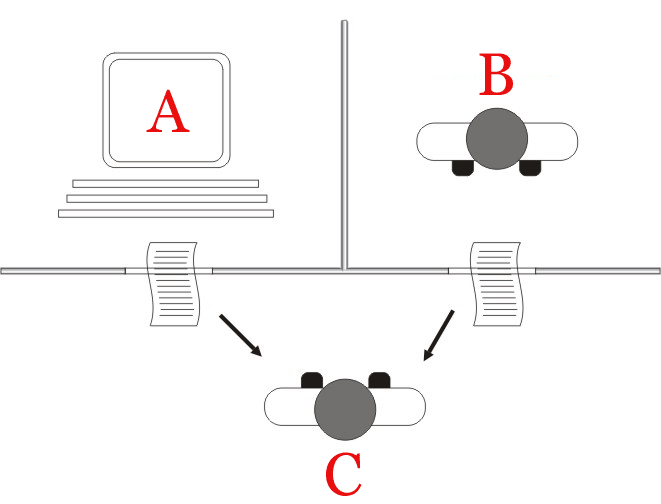
\includegraphics[scale=0.4]{turing.png}
\caption{Test de Turing}
\end{figure}
\subsubsection{Pensar como un humano: modelo cognitivo.}
Primero tenemos que penetrar en la mente humana para ver cómo funciona. Podemos hacerlo mediante \emph{introspección} (intentando atrapar nuestros propios pensamientos conforme van apareciendo) o mediante experimentos psicológicos. Una vez que contemos con una teoría precisa sobre el funcionamiento de la mente, podremos expresarla en un programa de computador. Si los datos de entrada/salida del programa y los tiempos de realización son parecidos, podremos concluir que algunos de los mecanismos del programa se pueden comparar con los que utilizamos los seres humanos.\\

La \textbf{ciencia cognitiva} es el campo interdisciplinar en el que convergen modelos computacionales de IA y técnicas experimentales de psicología para intentar elaborar teorías precisas y verificables sobre el funcionamiento de la mente humana.

\subsubsection{Pensamiento racional: ''leyes del pensamiento''.}

Está basada en la lógica de Aristóteles. Consiste en construir sistemas inteligentes que puedan resolver problemas (resolubles) a partir de un problema descrito en lenguaje lógico. \\

Sus dos mayores obstáculos son la dificultad de expresar conocimiento informal en lenguaje lógico y las limitaciones físicas de computación (agotamiento de recursos).

\subsubsection{Actuar de forma racional: agente racional.}

Un \textbf{agente} es algo que razona. Pero se espera que los programas informáticos tengan otros atributos que los diferencien de los convencionales, como que estén dotados de controles autónomos, que se adapten a los cambios, etc. Un \textbf{agente racional} es aquel que actúa con la intención de alcanzar el mejor resultado o, cuando hay incertidumbre, el mejor resultado esperado.\\

En el enfoque de la IA según las ''leyes del pensamiento'', todo el énfasis se pone en hacer inferencias correcctas.

\section{Tema 2. Agentes.}

Un \textbf{agente} es cualquier cosa capaz de percibir su medioambiente con ayuda de sensores y actuar en ese medio utilizando actuadores. Un agente humano tiene ojos, oídos y otros órganos sensoriales además de manos, boca, piernas y otras partes del cuerpor para actuar. Un agente robot recibe pulsaciones del teclado, archivos de ifnormación y paquetes via red a modo de entradas sensoriales y actúa sobre el medio con mensajes en el montior, escribiendo ficheros y enviando paquetes por la red. Se trabaja con la hipótesis de que cada agente puede percibir sus propias acciones (pero no siempres sus efectos).

\begin{figure}[H]
\centering
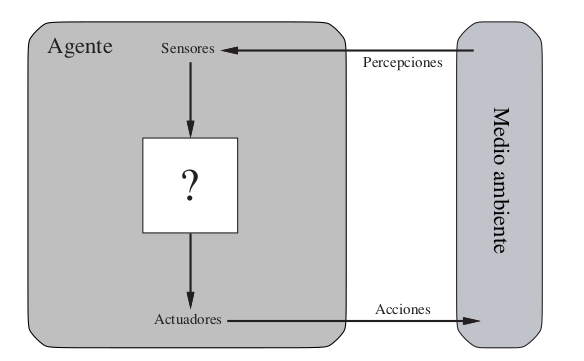
\includegraphics[scale=0.4]{agentes.png}
\caption{Funcionamiento de un agente.}
\end{figure}

La \textbf{percepción} se utiliza en este contexto para indicar que el agente puede recibir entradas en cualquier instante. La \textbf{secuencia de percepciones} de un agente refleja el historial completo de lo que ha recibido. En general, esta secuencia influirá en la decisión que tome el agente en un momento dado. En cierto modo, podemos afirmar que el comportamiento del agente viene dado por la \textbf{función del agente} que proyecta una percepción dada una acción.\\

La \textbf{Inteligencia Artificial} es el subcampo de la informática que se dedica a construir agentes que exhiban aspectos del comportamiento inteligente. \\

Un \textbf{agente inteligente} es un sistema de ordenador \emph{situado} en un entorno que es capaz de realizar acciones de forma \emph{autónoma} y que es \emph{flexible} para lograr los objetivos planteados.\\

\begin{itemize}
	\item \textbf{Situación}. El agente recibe entradas sensoriales de un entorno en el que está situado y realiza acciones que cambian dicho entorno.
	\item \textbf{Autonomía}. El sistema es capaz de actuar sin la intervención directa de los humanos y tiene control sobre sus propias acciones y estado interno.
	\item \textbf{Flexibilidad}
		\begin{itemize}
			\item \textbf{Reactivo}. El agente debe percibir el entorno y responder de forma temporal a los cambios que ocurran.
			\item \textbf{Pro-activo}. Los agentes no deben simplemente actuar en respuesta a su entorno, sino que deben exhibir comportamientos dirigidos a lograr objetivos y tomar la iniciativa cuando sea necesario.
			\item \textbf{Social}. Los agentes deben ser capaces de interactuar (cuando sea apropiado) con otros agentes artificiales o humanos para completar su propio proceso de resolución del probleam y ayudar a otros con sus actividades.
		\end{itemize}
\end{itemize}

Un \textbf{sistema basado en agentes} en un sistema en el que la abstracción clave utilizada es efectivamente el agente.

\subsection{Sistemas multiagente.}

Un \textbf{sistema multi-agente} es un sistema diseñado e implementado con varios agentes interactuando. Son interesantes para resolver problemas que tienen múltiples perspectivas, entidades o formas de ser resueltos.\\

Las características principales de un sistema multiagente son:
\begin{itemize}
	\item Cada agente tiene información incompleta o no todas las capacidades para resolver el problema, por lo que cada uno tiene un punto de vista limitado.
	\item No hay un sistema de control global.
	\item Los datos no están centralizados.
	\item La computación es asíncrona.
\end{itemize}

\subsection{Arquitecturas de agentes.}

\subsubsection{Arquitecturas deliberativas.}

\begin{itemize}
	\item \textbf{Sistema de símbolos físicos}. Conjunto de entidades físicas (símbolos) que pueden combinarse para formar estructuras y que es capaz de ejecutar procesos que operan con dichos símbolos de acuerdo a conjuntos de instrucciones codificadas simbólicamente.
	\item \textbf{Hipótesis de sistema de símbolos físicos}. Los sistemas de símbolos físicos son capaces de generar acciones inteligentes.
	\item \textbf{Agente deliberativo}. Es aquel que contiene un modelo simbólico del mundo explícitamente representado y cuyas decisiones se realizan a través de un razonamiento lógico basado en emparejamientos de patrones y manipulaciones simbólicas.
\end{itemize}

Sus principales problemas son el traslado del mundo real a una descripción simbólica en un tiempo razonable y la representación de entidades complejas del mundo real en lenguaje simbólico.

\subsubsection{Arquitecturas reactivas.}

El comportamiento inteligente de estas arquitecturas surge como resultado de la interacción del agente con su entorno. La inteligencia está en el ojo del espectador, no es una propiedad innata ni aislada.\\

Los agentes reactivos seleccionan las acciones sobre la base de las percepciones actuales, ignorando el resto de percepciones históricas. Ejemplo: un robot de limpieza.\\

Las representaciones del mundo pueden ser fundamentalmente de dos tipos:
\begin{itemize}
	\item \textbf{Icónicas}. Es una representación parcial del mundo, lo que nuestro agente es capaz de percibir.
	\item \textbf{Basadas en características}. Representación total del mundo.
\end{itemize}

\paragraph{Diseño de un agente reactivo}

EL flujo de interacción 	que debe seguir un agente reactivo es el siguiente:

\begin{enumerate}
	\item Percibir su entorno a través de sensores.
	\item Procesar la información percibida y realizar una representación interna de la misma.
	\item Escoger una acción de entre las posibles considerando la información percibida.
	\item Transformar la acción en señales para los actuadores y realizarla.
\end{enumerate}

\begin{figure}[H]
\centering
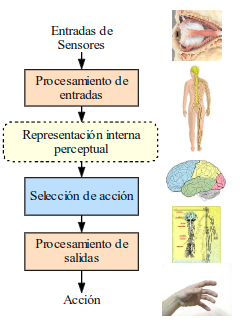
\includegraphics[scale=0.5]{flujo_ar.png}
\caption{Flujo de interacción de un agente reactivo}
\end{figure}
\newpage

\paragraph{Representación e implementación de funciones para seleccionar acciones.\\}

Para realizar la selección de acciones debemos construir una función sobre el vector de características que tenga $R$ valores de salida distintos, suponiendo que existen $R$ posibles acciones a elegir. Podemos representar e implementar estas funciones de varias formas:

\subparagraph{Sistemas de producción}

Proporcionan una representación adecuada para las funciones de selección de acciones. Una sistema de producción está formado por un conjunto de reglas (producciones). Cada producción se escribe de la siguiente manera: $c_i \rightarrow a_i$ donde $c_i$ es la condición y $a_i$ es la acción.\\

La condición de una relga puede ser cualquier función booleana definida sobre el vector de características. 

\subparagraph{Redes}

Consiste en implementar los sistemas de producción por medio de circuitos electrónicos (red de puertas lógicas). Las redes están formadas por elementos con umbral o cualquier otro elemento que aplique una función no lineal sobre una suma no ponderada de sus entradas. \\

Las funciones booleanas que se pueden implementar mediante una unidad lógica con umbral (ULU) se denominan \emph{funciones linealmente separables}.

\begin{figure}
\centering
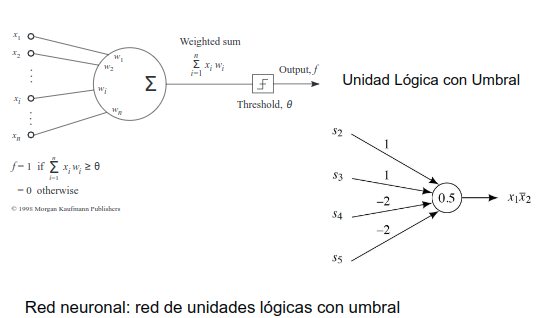
\includegraphics[scale=0.3]{redes.png}
\caption{Unidad lógica con umbral (ULU).}
\end{figure}

\subparagraph{Arquitectura de subsunción}

Consiste en hacer que el comportamiento global del agente descanse sobre un conjunto de módulos de comportamiento. Cada uno de ellos recibirá información directamente de las entradas sensoriales. Si estas entradas cumplen una precondición específica de cada módulo, se ejecutará un programa específico. Además, un módulo de comportamiento puede ser subsumido en otro.

\begin{figure}
\centering
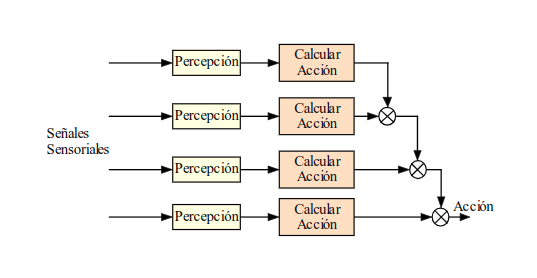
\includegraphics[scale=0.3]{subsuncion.png}
\caption{Arquitectura de subsunción.}
\end{figure}

\paragraph{Agentes reactivos con memoria}

Surgen para paliar nas limitaciones del sistema sensorial de un agente y mejorar la precisión teniendo en cuenta el historial sensorial.\\

En estos agentes, al representación de un estado en el instante $t+1$ depende de la representación del estado en el instante $t$ y la acción seleccionada en es momento.

Los agentes reactivos se diseñan completamente, por lo que es necesario anticipar todas las posibles reacciones para todas las situaciones. Realizan pocos cálculos y lo almacenan todo en memoria.


\section{Tema 3. Búsqueda en espacios de estados.}

\subsection{Diseño de un agente deliberativo.}

El agente dispone de varios elementos:
\begin{itemize}
	\item Un modelo del mundo en el que habita.
	\item Un modelo de los efectos de sus acciones sobre el mundo.
\end{itemize}

Nuestro agente será capaz de razonar sobre esos dos modelos para decidir qué hacer para conseguir un objetivo.

\subsection{La búsqueda en un espacio de estados.}

Un espacio de estados es una representación del conocimiento a través de las acciones del agente.\\
La búsqueda en el espacio de estados consiste en resolver el problema mediante la proyección de las distintas acciones que puede realizar nuestro agente. \\

Una estructura de \textbf{grafo dirigido} nos puede ser muy útil para buscar sencuencias de acciones que nos lleven al objetivo final. Un nodo representa un estado del sistema y una arista una posible acción. Esta estructura se denomina \textbf{grafo de estados}.

\begin{figure}
\centering
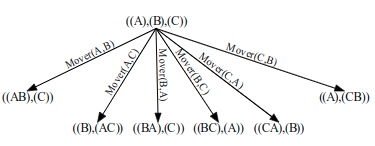
\includegraphics[scale=0.3]{grafo_estados.png}
\caption{Grafo de estados.}
\end{figure}







\end{document}
